%%%%%%%%%%%%%%%%%%%%%%%%%%%%%%%%%%%%%%%%%%%%%%%%%%%%%%%%%%
\section{Reinterpretation using Simplified Models}
\label{sec:ch5-smsReinterpretations}
%%%%%%%%%%%%%%%%%%%%%%%%%%%%%%%%%%%%%%%%%%%%%%%%%%%%%%%%%%

One of the possibilities for extending the experimental results from LLP
searches to a large variety of scenarios is through the use of simplified model topologies.
Simplified models (or simplified model spectra, SMS) have been widely used for the interpretation of
prompt and LLP searches. As discussed in Section~\ref{sec:simplifiedmodel}, a large
number of SMS topologies are possible for the distinct LLP signatures, which
can be grouped by the LLP production mode, decay and lifetime.
These SMS topologies aim to capture the main physical properties of the LLP
signal and can then be used to constraint other scenarios containing similar
topologies.
The use of simplified model results to constrain full models has been
shown to be possible~\cite{Kraml:2013mwa,Papucci:2014rja,Belanger:2015cra,Barducci:2015zna,Arina:2015uea,Ambrogi:2017lov}, 
even though it has its shortcomings~\cite{Ambrogi:2017lov}.
Also within the context of LLP searches, the use of
simplified model results for re-interpretation can be a good alternative, e.g.,
when a recasting based on a Monte Carlo simulation is difficult or
computationally too expensive.
In this Section we will briefly review how 
SMS results can be used to re-interpret searches for full
models as well as the particular challenges presented by LLP searches.
A concrete example of re-interpretation using simplified models is given in
Sec.~\ref{sec:ch5-smsHSCP}, based on the results of Ref.~\cite{Heisig:2015yla}.

\subsection{From Simplified to Full Models}

The interpretation of experimental results using
simplified models typically correspond to upper limits on the production
cross-section or signal efficiencies for a specific SMS topology (production and
decay channel). These results are provided as a function of the simplified model
parameters, which have been largely taken to be the masses of the BSM
particles appearing in the topology. For LLP topologies, however, 
a new parameter must be considered: the LLP lifetime (see Section~\ref{sec:simplifiedmodel}).
With the exception of searches for stable particles, the lifetime is one of the
main parameters affecting the topology efficiency and upper limit.

Once signal efficiencies\footnote{For simplicity we will refer to the signal
acceptance times efficiency as ``signal efficiency''. This efficiency
is a function of the simplified model parameters, including the LLP lifetime.}
($\epsilon$) are provided for one or more SMS topologies, these can be used, under some
approximations, to quickly compute the number of expected signal events ($S$)
for a full model:
\begin{equation}
S = \mathcal{L} \times \left( \sum_{\text{SMS}} \sigma_{\sms}
\times BR_{\sms} \times \epsilon_{\sms} \right) \, ,
\label{eq:decomp}
\end{equation}
where $\mathcal{L}$ is the luminosity for the respective search and the sum runs
over simplified model topologies. Since the production cross-section
($\sigma_{\sms}$) and branching ratios ($BR_{\sms}$) for each topology
can be quickly computed for any full model, the simplified model
signal efficiencies ($\epsilon_{\sms}$) can be directly used to
obtain the signal yield. This procedure does not rely
on any Monte Carlo simulation or recasting of LLP searches and
can be easily applied to a wide variety of models, if $\epsilon_{\sms}$
is known.
The main limitation of this approach comes from the limited (although
growing) number of SMS results available. Since $\epsilon_{\sms}$ is typically
known only for very few simplified models, the sum in eq.\ref{eq:decomp} is
limited to the number of available topologies, resulting in an underestimation of $S$.

For prompt SUSY searches a systematic approach for
re-interpreting simplified model results based on the procedure
outlined above has been developed in Refs.~\cite{Kraml:2013mwa,Papucci:2014rja}.
Furthermore, using the large number of available SUSY SMS results, 
public tools are available for constraining full models using these
results~\cite{Papucci:2014rja,Ambrogi:2017neo}.
Although no public tools are currently available for models with long-lived
particles, the same procedure can also be applied to LLP SMS results. This has
been shown in Ref.~\cite{Heisig:2015yla}, where,
using simplified model topologies, the 8~TeV CMS results for heavy
stable charged particles (HSCPs) have been used
to constrain regions of the CMSSM parameter space.
In the next section we review some of the results found in
Ref.~\cite{Heisig:2015yla}. Although these have been obtained within the
context of HSCPs, the main results can be generalized to other LLP
signatures and demonstrate some of the advantages and shortcomings of
re-interpretations using LLP simplified models.


\subsection{Reinterpretation using HSCP Simplified Models}
\label{sec:ch5-smsHSCP}

The CMS search for HSCPs in Ref.~\cite{Khachatryan:2015lla}
provided signal efficiencies for the simplified model topology:
$ pp \to \tilde{\tau} \tilde{\tau}$ as a function of the
stau mass. The stau is assumed to be stable (at detector scales), thus
producing a highly ionizing track, which can be used to search
for this scenario. Since the stau lifetime ($\tau$) is assumed to be $\gg
10$~ns, the signal efficiencies do not depend on $\tau$,
thus simplifying the SMS parameter space, which reduces to the stau
mass.\footnote{We point out that it is still possible to apply these simplified
model results to models with smaller LLP lifetimes if we include the suppression
factor from the LLP decay length distribution, as
discussed in Sec.~\ref{sec:ch5-validate}.
}
The relevant selection efficiencies required for a general purpose
Monte Carlo recasting of the HSCP search have also been provided by
the CMS analysis (see Sec.~\ref{sec:ch5-HSCPs} for details).


The efficiencies for the stau simplified model
can be used to constrain a full BSM scenario which contains
HSCPs. In Ref.~\cite{Heisig:2015yla} the region of the CMSSM parameter
space with $m_{\tilde \tau} - m_{\tilde \chi_1^0} < m_{\tau}$ has been
considered, since it provides a possible solution to the Lithium
problem~\cite{Spite:1982dd, Cyburt:2008kw}. Due to the small
mass difference, the stau is long-lived and decays outside the detector,
thus generating a HSCP signal.
In Fig.~\ref{fig:cmssmA} we show the constraint on the CMSSM parameter
space obtained using only the simplified model provided by CMS (direct stau
production).
Since the simplified model only contains one parameter it
translates to a limit on the stau mass ($m_{\tilde \tau} < 260$~GeV),
as shown by the blue region in the Figure.
In this CMSSM scenario, however, direct production of staus only contribute to a
small fraction of the total HSCP signal, since staus are typically produced from
cascade decays of heavier SUSY states, such as charginos, squarks and gluinos.
Furthermore, there are several possible topologies which contains a stau and the
LSP ($\tilde \chi_1^0$) in the final state, thus resulting in a
mixed missing energy-HSCP signature.
Therefore using only the CMS constraints for the direct stau production
simplified model largely underestimate the exclusion potential of the CMS
search. 


\begin{figure}[!h]
\centering
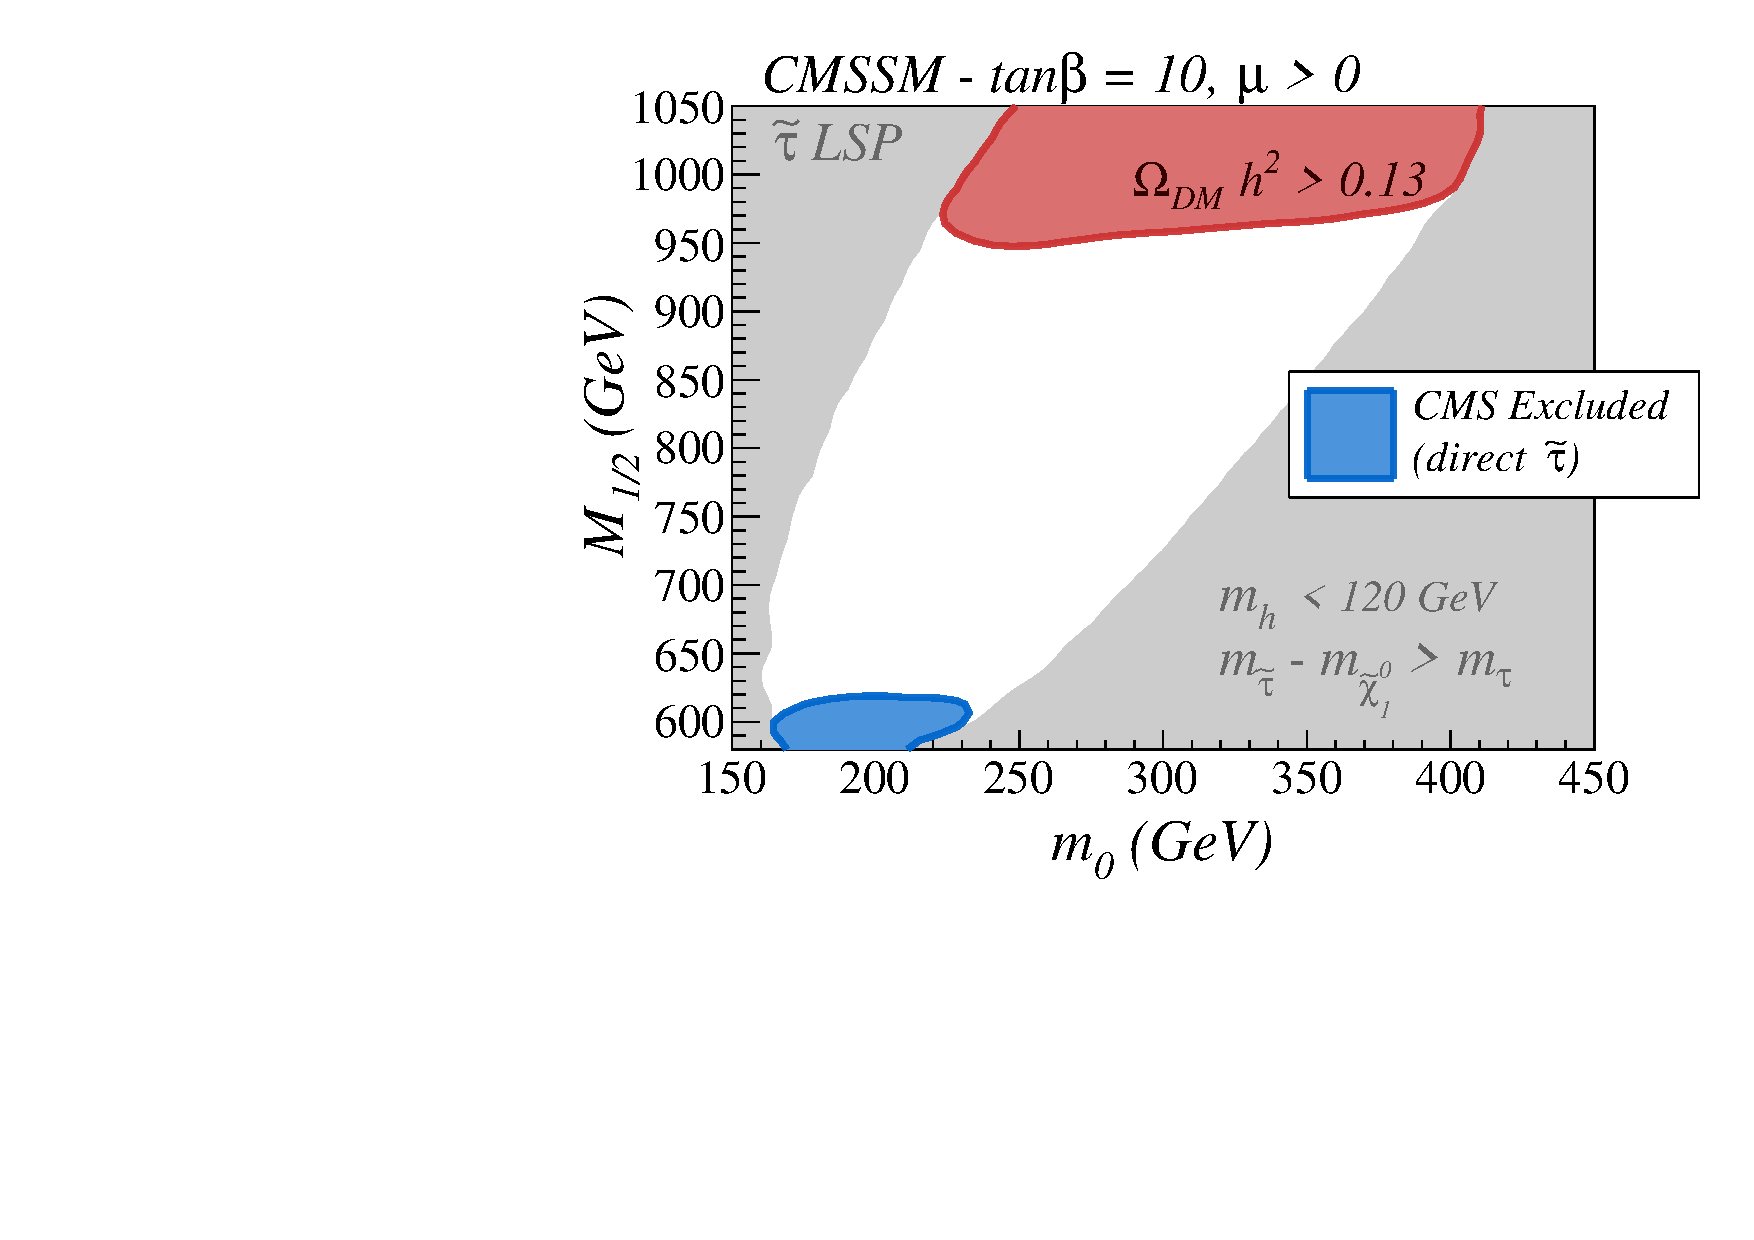
\includegraphics[width=0.8\textwidth]{ch5-figures/sms_exclusion_direct.pdf}
\caption{Region of the CMSSM parameter space with long-lived NLSP staus.
The light gray regions are excluded by the requirements $m_{\tilde \tau} \gtrsim
m_{\tilde \chi_1^0}$ and $ 120 \mbox{ GeV} \leq m_h \leq 130 \mbox{ GeV}$.
The top red region is excluded by the upper limit on the neutralino relic
density, while the lower blue region is excluded by the CMS constraints
on direct production of long-lived staus. For more details see Ref.~\cite{Heisig:2015yla}.
}
\label{fig:cmssmA}
\end{figure}


In order to improve the constraints shown in Fig,~\ref{fig:cmssmA}, one must
have efficiencies for several SMS topologies. Fortunately a Monte Carlo
recasting of the 8~TeV CMS search is possible (see Sec.~\ref{sec:ch5-HSCPs} for details)
and can be used to compute simplified model efficiencies.
In Ref.~\cite{Heisig:2015yla} seven additional simplified models (containing
cascade decays) were considered and their efficiencies computed as a function of
the masses appearing in the topology. A summary of the topologies considered
are shown in Table~\ref{tab:defModels}. It is important to point out that
it is not necessary to specify the Standard Model final states appearing in the
simplified models, since the HSCP search is inclusive and the efficiencies
do not depend on the additional event activity.
Using this extended database of simplified model efficiencies
and eq.~\ref{eq:decomp} we can compute a more inclusive signal yield for each
point of the CMSSM parameter space and improve the constraints on the model.
The results are shown in Fig.~\ref{fig:cmssmB}, where
we see a drastic improvement in the region excluded by
the constraints on HSCPs, as expected.
For this specific scenario (with
$\tan\beta = 10$), all the parameter space is excluded either by the CMS or dark matter
constraints~\cite{Heisig:2015yla}.


\begin{table}
\begin{center}
\begin{tabular}{lcc}
\toprule
SMS topology & Notation in Chapter~\ref{sec:simplifiedmodel}
% & parameters 
%& SUSY\;process
\\
\midrule
$pp \to X\;X$ & DPP
% & $m_{\text{HSCP}}$ 
% & $pp\to \charg \charg$ 
\\
$pp \to Y_1\;Y_1, Y_1\;\to SM\;X$ & HP
% & $m_{\text{HSCP}},m_{\text{prod}}$ 
%& $pp\to \sq\sq\to \charg \charg$ 
\\
$pp \to Y_1\;Y_1, Y_1\;\to SM\; Y_2, Y_2\;\to SM\;X$ & -
% & $m_{\text{HSCP}},m_{\text{int}},m_{\text{prod}}$ 
%& $pp\to \sq\sq\to \neu \neu\to\stau_1\stau_1$ 
\\
$pp \to Y_1\;Y_2, Y_1\;\to SM\;Y_2, Y_2\;\to SM\; X$ & -
% & $m_{\text{HSCP}},m_{\text{int}},m_{\text{prod}}$ 
%& $pp\to \neu\s\chi^\pm_2\to \stau_1 (\charg\to\stau_1)$ 
\\
$pp \to Y\;Y, Y\;\to SM\;SM\;X$ & HP
% & $m_{\text{HSCP}},m_{\text{prod}}$ 
%& $pp\to \sq\sq\to \stau_1\stau_1$ 
\\
$pp \to inv\; X$ & CC
% & $m_{\text{HSCP}} = m_{\text{inv}}$ 
%& $pp\to  \charg \neu$ 
\\
$pp \to Y_1\;Y_2, Y_1\;\to SM\;inv, Y_2\;\to SM\;X$ & -
% & $m_{\text{HSCP}},m_{\text{prod}}$
%&  $pp\to \sq\sq\to \charg \neu$ 
\\
$pp \to Y_1\;Y_2, Y_1\;\to SM\;inv, Y_2\;\to Y_3\;SM, Y_3\;\to SM\;X$ & -
% & $m_{\text{HSCP}},m_{\text{int}},m_{\text{prod}}$
%&  $pp\to \sq\sq\to \neu (\neu\to\stau_1)$ 
\\
\bottomrule
\end{tabular}
\end{center}
\caption{Definitions of the HSCP simplified models considered in this Section.
$X$ represents the HSCP, $Y_i$ represent intermediate BSM particles,
$SM$ represents any Standard Model particle and $inv$ represents an invisible
final state, such as the neutralino. The correspondance with the simplified models language 
of Chapter~\ref{sec:simplifiedmodel} (section~\ref{SM:secProduction_modes}) is also given.}
\label{tab:defModels}
\end{table}



\begin{figure}[!h]
\centering
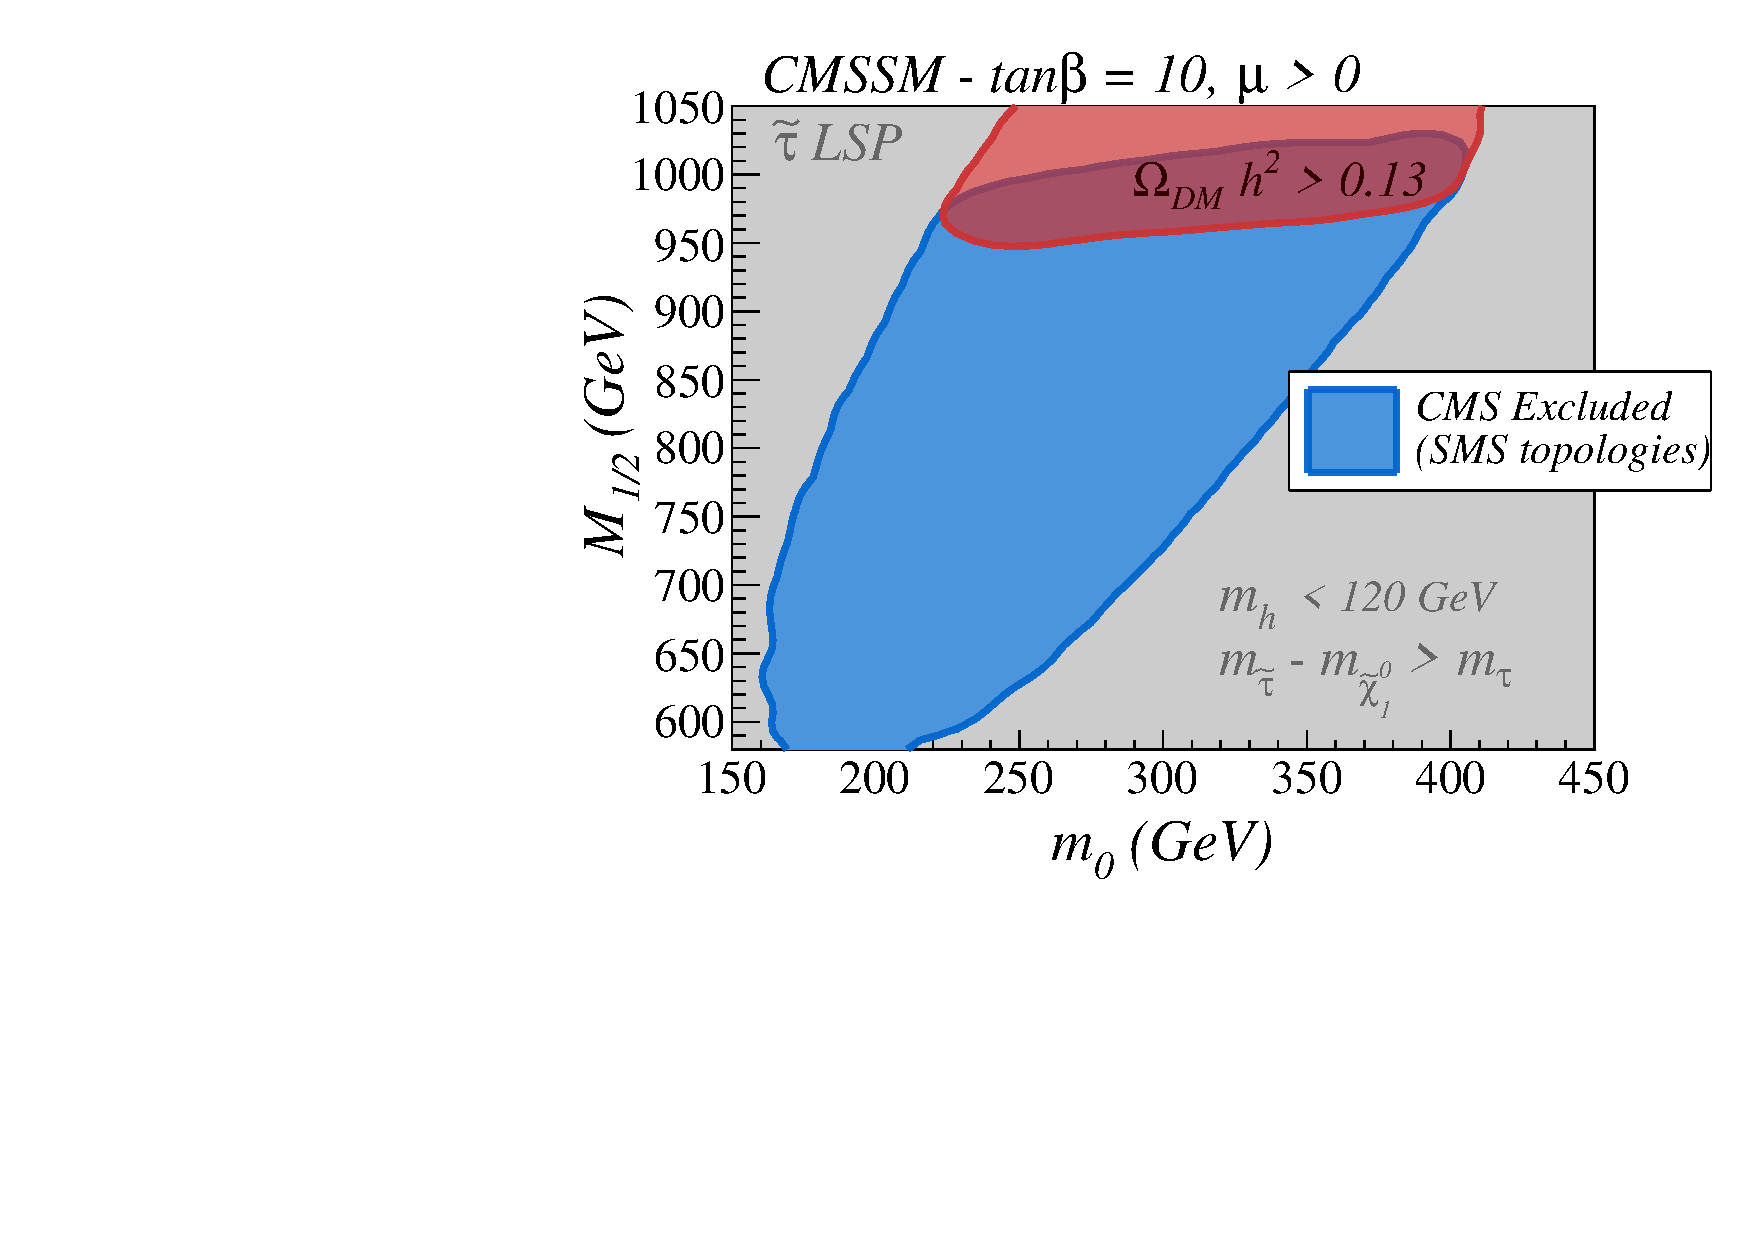
\includegraphics[width=0.8\textwidth]{ch5-figures/sms_exclusion_all.pdf}
\caption{Same as Fig.~\ref{fig:cmssmB}, but using all the simplified
models listed in Table~\ref{tab:defModels}.
}
\label{fig:cmssmB}
\end{figure}


Fig.~\ref{fig:cmssmB} illustrates the feasibility of using simplified
model efficiencies to constrain full models.
This approach has the advantage of being computationally inexpensive
(once the efficiencies are known) and can be used to quickly test
a large number of model points. However the approach relies on a few
approximations and is never fully inclusive, since the number of available SMS topologies is always limited.
Hence it is relevant to verify
how close the simplified model re-interpretation comes to the full recasting
using a Monte Carlo simulation.
In Ref.~\cite{Heisig:2015yla} it was shown that, within
the CMSSM scenario discussed above and using eight simplified model
topologies, the SMS results reproduce the full simulation within
20\% or better.
Since this error is of the order of the uncertainties in recasting,
the use of simplified models becomes a viable alternative to full recasting.
The SMS re-interpretation can become even more relevant for the cases
where a Monte Carlo recasting is not possible.


\vskip 0.1in
\noindent {\bf Lessons learned}
\vskip 0.1in

% The example discussed in Sec.~\ref{sec:ch5-smsHSCP} illustrates
% how simplified models for LLPs can be used as a re-interpretation tool.
% One important point which becomes clear once we compare Figs.~\ref{fig:cmssmA}
% and \ref{fig:cmssmB} is the importance of a sufficiently inclusive database
% of simplified model efficiencies. This can be provided by the experimental
% collaborations or generated by theory groups if a full recasting is available.
% Furthermore, since LLP searches can be very inclusive,
% the simplified models considered can also be defined
% inclusively, as discussed above.
% In this way a few number of simplified models can cover
% a large number of event topologies, thus increasing the SMS coverage
% of full models.


The example discussed in Sec.~\ref{sec:ch5-smsHSCP} illustrates how simplified
models for LLPs can be used as a re-interpretation tool. One important
point which becomes clear once we compare Figs.~\ref{fig:cmssmA} and~\ref{fig:cmssmB} 
is the importance of a sufficiently inclusive database of simplified 
model efficiencies. In particular, depending on the full BSM scenario considered,
the minimal set of simplified models proposed in Chapter~\ref{sec:simplifiedmodel} and 
Appendix~\ref{sec:library_more} may not be sufficient to allow for a re-interpretation 
based on simplified model results alone. In these cases results for additional simplified 
model topologies are necessary and can be provided by the experimental collaborations or 
generated by theory groups if a full recasting is available.
Furthermore, since LLP searches can be very inclusive,
the simplified models considered can also be defined inclusively,
as discussed above. In this way a limited number of simplified models
can cover a large number of event topologies, thus increasing the
SMS coverage of full models.


